\documentclass{standalone}
\usepackage{tikz}
\usetikzlibrary{patterns, positioning}
\usepackage[sfdefault]{ClearSans} %% option 'sfdefault' activates Clear Sans as the default text font
\usepackage[T1]{fontenc}

\begin{document}
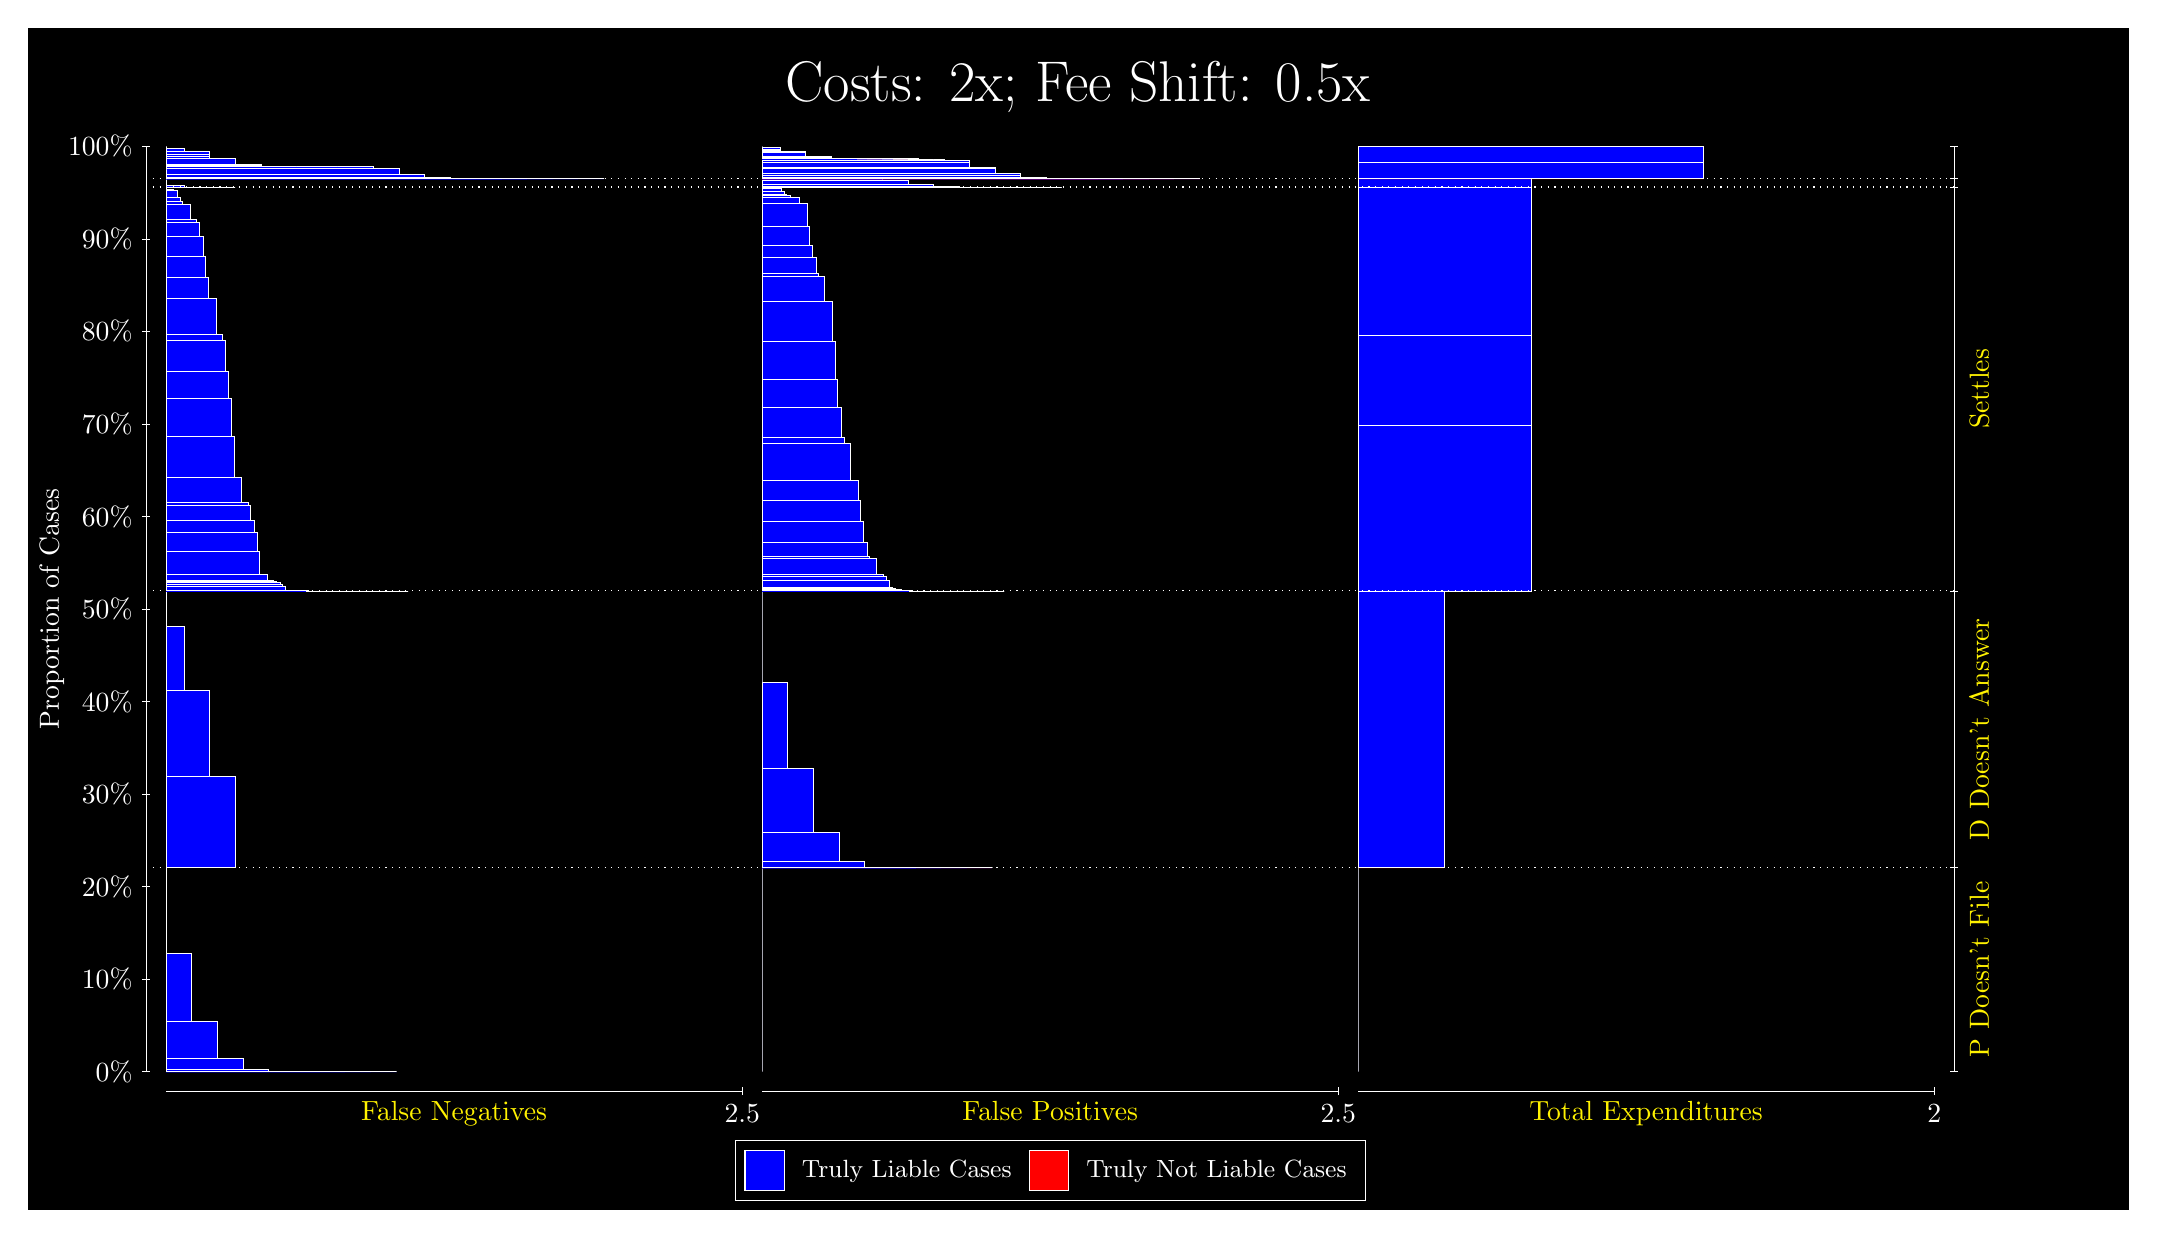
\begin{tikzpicture}
\draw[fill=black] (0,0) rectangle (26.667,15);
\draw[text=white] (0,13.5) rectangle (26.667,15) node[midway] {\huge Costs: 2x; Fee Shift: 0.5x};
\draw[white, very thin] (1.5,1.75) -- (1.5,13.5);
\node[rotate=90, text=white, anchor=center] at (0.3, 7.625) {Proportion of Cases};
\draw[white, very thin] (1.45,1.75) -- (1.55,1.75);
\node[text=white, anchor=east] at (1.45, 1.75) {0\%};
\draw[white, very thin] (1.45,2.925) -- (1.55,2.925);
\node[text=white, anchor=east] at (1.45, 2.925) {10\%};
\draw[white, very thin] (1.45,4.1) -- (1.55,4.1);
\node[text=white, anchor=east] at (1.45, 4.1) {20\%};
\draw[white, very thin] (1.45,5.275) -- (1.55,5.275);
\node[text=white, anchor=east] at (1.45, 5.275) {30\%};
\draw[white, very thin] (1.45,6.45) -- (1.55,6.45);
\node[text=white, anchor=east] at (1.45, 6.45) {40\%};
\draw[white, very thin] (1.45,7.625) -- (1.55,7.625);
\node[text=white, anchor=east] at (1.45, 7.625) {50\%};
\draw[white, very thin] (1.45,8.8) -- (1.55,8.8);
\node[text=white, anchor=east] at (1.45, 8.8) {60\%};
\draw[white, very thin] (1.45,9.975) -- (1.55,9.975);
\node[text=white, anchor=east] at (1.45, 9.975) {70\%};
\draw[white, very thin] (1.45,11.15) -- (1.55,11.15);
\node[text=white, anchor=east] at (1.45, 11.15) {80\%};
\draw[white, very thin] (1.45,12.325) -- (1.55,12.325);
\node[text=white, anchor=east] at (1.45, 12.325) {90\%};
\draw[white, very thin] (1.45,13.5) -- (1.55,13.5);
\node[text=white, anchor=east] at (1.45, 13.5) {100\%};

\draw[white, very thin] (24.457,1.75) -- (24.457,13.5);
\draw[white, very thin] (24.407,1.75) -- (24.507,1.75);
\node[anchor=west] at (24.407, 1.75) {};
\draw[white, very thin] (24.407,4.3399) -- (24.507,4.3399);
\node[anchor=west] at (24.407, 4.3399) {};
\draw[white, very thin] (24.407,7.8535) -- (24.507,7.8535);
\node[anchor=west] at (24.407, 7.8535) {};
\draw[white, very thin] (24.407,12.984) -- (24.507,12.984);
\node[anchor=west] at (24.407, 12.984) {};
\draw[white, very thin] (24.407,13.091) -- (24.507,13.091);
\node[anchor=west] at (24.407, 13.091) {};
\draw[white, very thin] (24.407,13.5) -- (24.507,13.5);
\node[anchor=west] at (24.407, 13.5) {};

\draw[white, very thin, fill=blue] (1.75,1.75) rectangle (4.6775,1.75);
\draw[white, very thin, fill=blue] (1.75,1.75) rectangle (4.3523,1.75);
\draw[white, very thin, fill=blue] (1.75,1.75) rectangle (4.027,1.75);
\draw[white, very thin, fill=blue] (1.75,1.75) rectangle (3.7017,1.7501);
\draw[white, very thin, fill=blue] (1.75,1.7501) rectangle (3.3764,1.7521);
\draw[white, very thin, fill=blue] (1.75,1.7521) rectangle (3.0511,1.7768);
\draw[white, very thin, fill=blue] (1.75,1.7768) rectangle (2.7258,1.9244);
\draw[white, very thin, fill=blue] (1.75,1.9244) rectangle (2.4006,2.3924);
\draw[white, very thin, fill=blue] (1.75,2.3924) rectangle (2.0753,3.2532);
\draw[white, very thin, fill=red] (1.75,3.2532) rectangle (1.75,3.2532);
\draw[white, very thin, fill=blue] (1.75,3.2532) rectangle (1.75,4.3399);
\draw[white, very thin, fill=blue] (1.75,4.3399) rectangle (2.6283,5.5043);
\draw[white, very thin, fill=blue] (1.75,5.5043) rectangle (2.303,6.5952);
\draw[white, very thin, fill=blue] (1.75,6.5952) rectangle (1.9777,7.4054);
\draw[white, very thin, fill=red] (1.75,7.4054) rectangle (1.75,7.4054);
\draw[white, very thin, fill=blue] (1.75,7.4054) rectangle (1.75,7.8535);
\draw[white, very thin, fill=blue] (1.75,7.8535) rectangle (4.8239,7.8535);
\draw[white, very thin, fill=blue] (1.75,7.8535) rectangle (4.5312,7.8535);
\draw[white, very thin, fill=blue] (1.75,7.8535) rectangle (4.4986,7.8535);
\draw[white, very thin, fill=blue] (1.75,7.8535) rectangle (4.2384,7.8535);
\draw[white, very thin, fill=blue] (1.75,7.8535) rectangle (4.2059,7.8535);
\draw[white, very thin, fill=blue] (1.75,7.8535) rectangle (4.1734,7.8535);
\draw[white, very thin, fill=blue] (1.75,7.8535) rectangle (4.092,7.8535);
\draw[white, very thin, fill=blue] (1.75,7.8535) rectangle (3.9131,7.8535);
\draw[white, very thin, fill=blue] (1.75,7.8535) rectangle (3.8806,7.8535);
\draw[white, very thin, fill=blue] (1.75,7.8535) rectangle (3.8481,7.8535);
\draw[white, very thin, fill=blue] (1.75,7.8535) rectangle (3.7993,7.8535);
\draw[white, very thin, fill=blue] (1.75,7.8535) rectangle (3.7668,7.8535);
\draw[white, very thin, fill=blue] (1.75,7.8535) rectangle (3.5878,7.8552);
\draw[white, very thin, fill=blue] (1.75,7.8552) rectangle (3.5553,7.8561);
\draw[white, very thin, fill=blue] (1.75,7.8561) rectangle (3.5228,7.8564);
\draw[white, very thin, fill=blue] (1.75,7.8564) rectangle (3.474,7.857);
\draw[white, very thin, fill=blue] (1.75,7.857) rectangle (3.4415,7.857);
\draw[white, very thin, fill=blue] (1.75,7.857) rectangle (3.3602,7.8675);
\draw[white, very thin, fill=blue] (1.75,7.8675) rectangle (3.2626,7.912);
\draw[white, very thin, fill=blue] (1.75,7.912) rectangle (3.23,7.9425);
\draw[white, very thin, fill=blue] (1.75,7.9425) rectangle (3.1975,7.9581);
\draw[white, very thin, fill=blue] (1.75,7.9581) rectangle (3.1487,7.9806);
\draw[white, very thin, fill=blue] (1.75,7.9806) rectangle (3.1162,7.9847);
\draw[white, very thin, fill=blue] (1.75,7.9847) rectangle (3.0349,8.0661);
\draw[white, very thin, fill=blue] (1.75,8.0661) rectangle (2.9373,8.3565);
\draw[white, very thin, fill=blue] (1.75,8.3565) rectangle (2.9048,8.5948);
\draw[white, very thin, fill=blue] (1.75,8.5948) rectangle (2.8722,8.7452);
\draw[white, very thin, fill=blue] (1.75,8.7452) rectangle (2.8234,8.9435);
\draw[white, very thin, fill=blue] (1.75,8.9435) rectangle (2.7909,8.984);
\draw[white, very thin, fill=blue] (1.75,8.984) rectangle (2.7096,9.3012);
\draw[white, very thin, fill=blue] (1.75,9.3012) rectangle (2.612,9.8158);
\draw[white, very thin, fill=blue] (1.75,9.8158) rectangle (2.5795,10.296);
\draw[white, very thin, fill=blue] (1.75,10.296) rectangle (2.5469,10.647);
\draw[white, very thin, fill=blue] (1.75,10.647) rectangle (2.4982,11.032);
\draw[white, very thin, fill=blue] (1.75,11.032) rectangle (2.4656,11.114);
\draw[white, very thin, fill=blue] (1.75,11.114) rectangle (2.3843,11.575);
\draw[white, very thin, fill=blue] (1.75,11.575) rectangle (2.2867,11.831);
\draw[white, very thin, fill=blue] (1.75,11.831) rectangle (2.2542,12.105);
\draw[white, very thin, fill=blue] (1.75,12.105) rectangle (2.2217,12.362);
\draw[white, very thin, fill=blue] (1.75,12.362) rectangle (2.1729,12.539);
\draw[white, very thin, fill=blue] (1.75,12.539) rectangle (2.1403,12.573);
\draw[white, very thin, fill=blue] (1.75,12.573) rectangle (2.059,12.769);
\draw[white, very thin, fill=blue] (1.75,12.769) rectangle (1.9614,12.803);
\draw[white, very thin, fill=blue] (1.75,12.803) rectangle (1.9289,12.852);
\draw[white, very thin, fill=blue] (1.75,12.852) rectangle (1.8964,12.937);
\draw[white, very thin, fill=blue] (1.75,12.937) rectangle (1.8476,12.955);
\draw[white, very thin, fill=blue] (1.75,12.955) rectangle (1.8151,12.958);
\draw[white, very thin, fill=red] (1.75,12.958) rectangle (1.75,12.958);
\draw[white, very thin, fill=blue] (1.75,12.958) rectangle (1.75,12.984);
\draw[white, very thin, fill=blue] (1.75,12.984) rectangle (2.6283,12.984);
\draw[white, very thin, fill=blue] (1.75,12.984) rectangle (2.303,12.985);
\draw[white, very thin, fill=blue] (1.75,12.985) rectangle (1.9777,13.002);
\draw[white, very thin, fill=red] (1.75,13.002) rectangle (1.75,13.002);
\draw[white, very thin, fill=blue] (1.75,13.002) rectangle (1.75,13.091);
\draw[white, very thin, fill=blue] (1.75,13.091) rectangle (7.3123,13.091);
\draw[white, very thin, fill=blue] (1.75,13.091) rectangle (6.9871,13.091);
\draw[white, very thin, fill=blue] (1.75,13.091) rectangle (6.6618,13.091);
\draw[white, very thin, fill=blue] (1.75,13.091) rectangle (6.3365,13.091);
\draw[white, very thin, fill=blue] (1.75,13.091) rectangle (6.3365,13.091);
\draw[white, very thin, fill=blue] (1.75,13.091) rectangle (6.0112,13.091);
\draw[white, very thin, fill=blue] (1.75,13.091) rectangle (6.0112,13.091);
\draw[white, very thin, fill=blue] (1.75,13.091) rectangle (5.6859,13.091);
\draw[white, very thin, fill=blue] (1.75,13.091) rectangle (5.6859,13.094);
\draw[white, very thin, fill=blue] (1.75,13.094) rectangle (5.3606,13.101);
\draw[white, very thin, fill=blue] (1.75,13.101) rectangle (5.3606,13.107);
\draw[white, very thin, fill=blue] (1.75,13.107) rectangle (5.0354,13.141);
\draw[white, very thin, fill=blue] (1.75,13.141) rectangle (5.0354,13.151);
\draw[white, very thin, fill=blue] (1.75,13.151) rectangle (4.7101,13.216);
\draw[white, very thin, fill=blue] (1.75,13.216) rectangle (4.58,13.216);
\draw[white, very thin, fill=blue] (1.75,13.216) rectangle (4.3848,13.246);
\draw[white, very thin, fill=blue] (1.75,13.246) rectangle (4.2547,13.246);
\draw[white, very thin, fill=blue] (1.75,13.246) rectangle (4.2547,13.246);
\draw[white, very thin, fill=blue] (1.75,13.246) rectangle (4.0595,13.246);
\draw[white, very thin, fill=blue] (1.75,13.246) rectangle (4.0595,13.249);
\draw[white, very thin, fill=blue] (1.75,13.249) rectangle (3.9294,13.249);
\draw[white, very thin, fill=blue] (1.75,13.249) rectangle (3.7342,13.249);
\draw[white, very thin, fill=blue] (1.75,13.249) rectangle (3.7342,13.249);
\draw[white, very thin, fill=blue] (1.75,13.249) rectangle (3.6041,13.249);
\draw[white, very thin, fill=blue] (1.75,13.249) rectangle (3.4089,13.249);
\draw[white, very thin, fill=blue] (1.75,13.249) rectangle (3.2788,13.25);
\draw[white, very thin, fill=blue] (1.75,13.25) rectangle (3.2788,13.251);
\draw[white, very thin, fill=blue] (1.75,13.251) rectangle (3.0837,13.251);
\draw[white, very thin, fill=blue] (1.75,13.251) rectangle (2.9535,13.251);
\draw[white, very thin, fill=blue] (1.75,13.251) rectangle (2.9535,13.253);
\draw[white, very thin, fill=blue] (1.75,13.253) rectangle (2.9535,13.261);
\draw[white, very thin, fill=blue] (1.75,13.261) rectangle (2.9535,13.273);
\draw[white, very thin, fill=blue] (1.75,13.273) rectangle (2.6283,13.273);
\draw[white, very thin, fill=blue] (1.75,13.273) rectangle (2.6283,13.351);
\draw[white, very thin, fill=blue] (1.75,13.351) rectangle (2.303,13.353);
\draw[white, very thin, fill=blue] (1.75,13.353) rectangle (2.303,13.377);
\draw[white, very thin, fill=blue] (1.75,13.377) rectangle (2.303,13.405);
\draw[white, very thin, fill=blue] (1.75,13.405) rectangle (2.303,13.435);
\draw[white, very thin, fill=blue] (1.75,13.435) rectangle (1.9777,13.442);
\draw[white, very thin, fill=blue] (1.75,13.442) rectangle (1.9777,13.471);
\draw[white, very thin, fill=blue] (1.75,13.471) rectangle (1.9777,13.481);
\draw[white, very thin, fill=red] (1.75,13.481) rectangle (1.75,13.481);
\draw[white, very thin, fill=blue] (1.75,13.481) rectangle (1.75,13.5);
\draw[white, very thin, fill=red] (9.3189,1.75) rectangle (9.3189,1.75);
\draw[white, very thin, fill=blue] (9.3189,1.75) rectangle (9.3189,4.3399);
\draw[white, very thin, fill=red] (9.3189,4.3399) rectangle (12.246,4.3399);
\draw[white, very thin, fill=blue] (9.3189,4.3399) rectangle (12.246,4.3399);
\draw[white, very thin, fill=blue] (9.3189,4.3399) rectangle (11.921,4.3399);
\draw[white, very thin, fill=blue] (9.3189,4.3399) rectangle (11.596,4.3399);
\draw[white, very thin, fill=blue] (9.3189,4.3399) rectangle (11.271,4.3401);
\draw[white, very thin, fill=blue] (9.3189,4.3401) rectangle (10.945,4.3473);
\draw[white, very thin, fill=blue] (9.3189,4.3473) rectangle (10.62,4.4256);
\draw[white, very thin, fill=blue] (9.3189,4.4256) rectangle (10.295,4.7879);
\draw[white, very thin, fill=blue] (9.3189,4.7879) rectangle (9.9694,5.5981);
\draw[white, very thin, fill=blue] (9.3189,5.5981) rectangle (9.6442,6.689);
\draw[white, very thin, fill=blue] (9.3189,6.689) rectangle (9.3189,7.8535);
\draw[white, very thin, fill=red] (9.3189,7.8535) rectangle (12.393,7.8535);
\draw[white, very thin, fill=blue] (9.3189,7.8535) rectangle (12.393,7.8535);
\draw[white, very thin, fill=blue] (9.3189,7.8535) rectangle (12.068,7.8535);
\draw[white, very thin, fill=red] (9.3189,7.8535) rectangle (11.954,7.8535);
\draw[white, very thin, fill=blue] (9.3189,7.8535) rectangle (11.954,7.8535);
\draw[white, very thin, fill=blue] (9.3189,7.8535) rectangle (11.742,7.8535);
\draw[white, very thin, fill=red] (9.3189,7.8535) rectangle (11.661,7.8535);
\draw[white, very thin, fill=blue] (9.3189,7.8535) rectangle (11.661,7.8535);
\draw[white, very thin, fill=blue] (9.3189,7.8535) rectangle (11.628,7.8535);
\draw[white, very thin, fill=red] (9.3189,7.8535) rectangle (11.515,7.8535);
\draw[white, very thin, fill=blue] (9.3189,7.8535) rectangle (11.515,7.8535);
\draw[white, very thin, fill=blue] (9.3189,7.8535) rectangle (11.417,7.8539);
\draw[white, very thin, fill=blue] (9.3189,7.8539) rectangle (11.336,7.854);
\draw[white, very thin, fill=blue] (9.3189,7.854) rectangle (11.303,7.8544);
\draw[white, very thin, fill=red] (9.3189,7.8544) rectangle (11.222,7.8544);
\draw[white, very thin, fill=blue] (9.3189,7.8544) rectangle (11.222,7.8578);
\draw[white, very thin, fill=blue] (9.3189,7.8578) rectangle (11.189,7.859);
\draw[white, very thin, fill=blue] (9.3189,7.859) rectangle (11.092,7.8791);
\draw[white, very thin, fill=blue] (9.3189,7.8791) rectangle (11.01,7.8821);
\draw[white, very thin, fill=blue] (9.3189,7.8821) rectangle (10.978,7.9003);
\draw[white, very thin, fill=red] (9.3189,7.9003) rectangle (10.929,7.9003);
\draw[white, very thin, fill=blue] (9.3189,7.9003) rectangle (10.929,7.9849);
\draw[white, very thin, fill=blue] (9.3189,7.9849) rectangle (10.896,8.0337);
\draw[white, very thin, fill=blue] (9.3189,8.0337) rectangle (10.864,8.068);
\draw[white, very thin, fill=blue] (9.3189,8.068) rectangle (10.766,8.2636);
\draw[white, very thin, fill=blue] (9.3189,8.2636) rectangle (10.685,8.2979);
\draw[white, very thin, fill=blue] (9.3189,8.2979) rectangle (10.653,8.4747);
\draw[white, very thin, fill=blue] (9.3189,8.4747) rectangle (10.604,8.7322);
\draw[white, very thin, fill=blue] (9.3189,8.7322) rectangle (10.571,9.0063);
\draw[white, very thin, fill=blue] (9.3189,9.0063) rectangle (10.539,9.2621);
\draw[white, very thin, fill=blue] (9.3189,9.2621) rectangle (10.441,9.7233);
\draw[white, very thin, fill=blue] (9.3189,9.7233) rectangle (10.36,9.8052);
\draw[white, very thin, fill=blue] (9.3189,9.8052) rectangle (10.327,10.19);
\draw[white, very thin, fill=blue] (9.3189,10.19) rectangle (10.278,10.541);
\draw[white, very thin, fill=blue] (9.3189,10.541) rectangle (10.246,11.021);
\draw[white, very thin, fill=blue] (9.3189,11.021) rectangle (10.213,11.536);
\draw[white, very thin, fill=blue] (9.3189,11.536) rectangle (10.116,11.853);
\draw[white, very thin, fill=blue] (9.3189,11.853) rectangle (10.034,11.894);
\draw[white, very thin, fill=blue] (9.3189,11.894) rectangle (10.002,12.092);
\draw[white, very thin, fill=blue] (9.3189,12.092) rectangle (9.9532,12.242);
\draw[white, very thin, fill=blue] (9.3189,12.242) rectangle (9.9206,12.48);
\draw[white, very thin, fill=blue] (9.3189,12.48) rectangle (9.8881,12.771);
\draw[white, very thin, fill=blue] (9.3189,12.771) rectangle (9.7905,12.852);
\draw[white, very thin, fill=blue] (9.3189,12.852) rectangle (9.7092,12.856);
\draw[white, very thin, fill=blue] (9.3189,12.856) rectangle (9.6767,12.879);
\draw[white, very thin, fill=blue] (9.3189,12.879) rectangle (9.6279,12.895);
\draw[white, very thin, fill=blue] (9.3189,12.895) rectangle (9.5954,12.925);
\draw[white, very thin, fill=blue] (9.3189,12.925) rectangle (9.5628,12.97);
\draw[white, very thin, fill=blue] (9.3189,12.97) rectangle (9.4652,12.98);
\draw[white, very thin, fill=blue] (9.3189,12.98) rectangle (9.3839,12.98);
\draw[white, very thin, fill=blue] (9.3189,12.98) rectangle (9.3514,12.981);
\draw[white, very thin, fill=blue] (9.3189,12.981) rectangle (9.3189,12.984);
\draw[white, very thin, fill=red] (9.3189,12.984) rectangle (13.125,12.984);
\draw[white, very thin, fill=blue] (9.3189,12.984) rectangle (13.125,12.984);
\draw[white, very thin, fill=blue] (9.3189,12.984) rectangle (12.799,12.984);
\draw[white, very thin, fill=blue] (9.3189,12.984) rectangle (12.474,12.984);
\draw[white, very thin, fill=blue] (9.3189,12.984) rectangle (12.149,12.984);
\draw[white, very thin, fill=blue] (9.3189,12.984) rectangle (11.824,12.989);
\draw[white, very thin, fill=blue] (9.3189,12.989) rectangle (11.498,13.024);
\draw[white, very thin, fill=blue] (9.3189,13.024) rectangle (11.173,13.073);
\draw[white, very thin, fill=blue] (9.3189,13.073) rectangle (10.848,13.089);
\draw[white, very thin, fill=blue] (9.3189,13.089) rectangle (10.522,13.091);
\draw[white, very thin, fill=blue] (9.3189,13.091) rectangle (10.197,13.091);
\draw[white, very thin, fill=red] (9.3189,13.091) rectangle (14.881,13.091);
\draw[white, very thin, fill=blue] (9.3189,13.091) rectangle (14.881,13.091);
\draw[white, very thin, fill=red] (9.3189,13.091) rectangle (14.556,13.091);
\draw[white, very thin, fill=blue] (9.3189,13.091) rectangle (14.556,13.091);
\draw[white, very thin, fill=red] (9.3189,13.091) rectangle (14.231,13.091);
\draw[white, very thin, fill=blue] (9.3189,13.091) rectangle (14.231,13.091);
\draw[white, very thin, fill=blue] (9.3189,13.091) rectangle (13.905,13.091);
\draw[white, very thin, fill=red] (9.3189,13.091) rectangle (13.905,13.091);
\draw[white, very thin, fill=blue] (9.3189,13.091) rectangle (13.905,13.091);
\draw[white, very thin, fill=red] (9.3189,13.091) rectangle (13.58,13.091);
\draw[white, very thin, fill=blue] (9.3189,13.091) rectangle (13.58,13.091);
\draw[white, very thin, fill=blue] (9.3189,13.091) rectangle (13.58,13.092);
\draw[white, very thin, fill=red] (9.3189,13.092) rectangle (13.255,13.092);
\draw[white, very thin, fill=blue] (9.3189,13.092) rectangle (13.255,13.094);
\draw[white, very thin, fill=blue] (9.3189,13.094) rectangle (13.255,13.094);
\draw[white, very thin, fill=blue] (9.3189,13.094) rectangle (12.93,13.098);
\draw[white, very thin, fill=red] (9.3189,13.098) rectangle (12.93,13.098);
\draw[white, very thin, fill=blue] (9.3189,13.098) rectangle (12.93,13.11);
\draw[white, very thin, fill=blue] (9.3189,13.11) rectangle (12.604,13.132);
\draw[white, very thin, fill=blue] (9.3189,13.132) rectangle (12.604,13.156);
\draw[white, very thin, fill=blue] (9.3189,13.156) rectangle (12.279,13.215);
\draw[white, very thin, fill=blue] (9.3189,13.215) rectangle (12.279,13.24);
\draw[white, very thin, fill=blue] (9.3189,13.24) rectangle (11.954,13.302);
\draw[white, very thin, fill=blue] (9.3189,13.302) rectangle (11.954,13.319);
\draw[white, very thin, fill=blue] (9.3189,13.319) rectangle (11.628,13.33);
\draw[white, very thin, fill=blue] (9.3189,13.33) rectangle (11.628,13.339);
\draw[white, very thin, fill=blue] (9.3189,13.339) rectangle (11.628,13.341);
\draw[white, very thin, fill=red] (9.3189,13.341) rectangle (11.498,13.341);
\draw[white, very thin, fill=blue] (9.3189,13.341) rectangle (11.498,13.341);
\draw[white, very thin, fill=blue] (9.3189,13.341) rectangle (11.303,13.341);
\draw[white, very thin, fill=blue] (9.3189,13.341) rectangle (11.303,13.342);
\draw[white, very thin, fill=red] (9.3189,13.342) rectangle (11.173,13.342);
\draw[white, very thin, fill=blue] (9.3189,13.342) rectangle (11.173,13.342);
\draw[white, very thin, fill=blue] (9.3189,13.342) rectangle (10.978,13.342);
\draw[white, very thin, fill=blue] (9.3189,13.342) rectangle (10.978,13.342);
\draw[white, very thin, fill=blue] (9.3189,13.342) rectangle (10.978,13.342);
\draw[white, very thin, fill=blue] (9.3189,13.342) rectangle (10.848,13.342);
\draw[white, very thin, fill=red] (9.3189,13.342) rectangle (10.848,13.342);
\draw[white, very thin, fill=blue] (9.3189,13.342) rectangle (10.848,13.342);
\draw[white, very thin, fill=blue] (9.3189,13.342) rectangle (10.653,13.342);
\draw[white, very thin, fill=blue] (9.3189,13.342) rectangle (10.653,13.342);
\draw[white, very thin, fill=blue] (9.3189,13.342) rectangle (10.522,13.343);
\draw[white, very thin, fill=red] (9.3189,13.343) rectangle (10.522,13.343);
\draw[white, very thin, fill=blue] (9.3189,13.343) rectangle (10.522,13.344);
\draw[white, very thin, fill=blue] (9.3189,13.344) rectangle (10.522,13.345);
\draw[white, very thin, fill=blue] (9.3189,13.345) rectangle (10.327,13.345);
\draw[white, very thin, fill=blue] (9.3189,13.345) rectangle (10.197,13.359);
\draw[white, very thin, fill=red] (9.3189,13.359) rectangle (10.197,13.359);
\draw[white, very thin, fill=blue] (9.3189,13.359) rectangle (10.197,13.363);
\draw[white, very thin, fill=blue] (9.3189,13.363) rectangle (10.197,13.375);
\draw[white, very thin, fill=blue] (9.3189,13.375) rectangle (10.002,13.375);
\draw[white, very thin, fill=blue] (9.3189,13.375) rectangle (9.8718,13.421);
\draw[white, very thin, fill=blue] (9.3189,13.421) rectangle (9.8718,13.44);
\draw[white, very thin, fill=blue] (9.3189,13.44) rectangle (9.5466,13.446);
\draw[white, very thin, fill=blue] (9.3189,13.446) rectangle (9.5466,13.461);
\draw[white, very thin, fill=blue] (9.3189,13.461) rectangle (9.5466,13.484);
\draw[white, very thin, fill=blue] (9.3189,13.484) rectangle (9.3189,13.5);
\draw[white, very thin, fill=red] (16.888,1.75) rectangle (16.888,1.75);
\draw[white, very thin, fill=blue] (16.888,1.75) rectangle (16.888,4.3399);
\draw[white, very thin, fill=red] (16.888,4.3399) rectangle (17.986,4.3399);
\draw[white, very thin, fill=blue] (16.888,4.3399) rectangle (17.986,7.8535);
\draw[white, very thin, fill=red] (16.888,7.8535) rectangle (19.083,7.8535);
\draw[white, very thin, fill=blue] (16.888,7.8535) rectangle (19.083,9.9628);
\draw[white, very thin, fill=red] (16.888,9.9628) rectangle (19.083,9.9628);
\draw[white, very thin, fill=blue] (16.888,9.9628) rectangle (19.083,11.105);
\draw[white, very thin, fill=red] (16.888,11.105) rectangle (19.083,11.105);
\draw[white, very thin, fill=blue] (16.888,11.105) rectangle (19.083,12.984);
\draw[white, very thin, fill=red] (16.888,12.984) rectangle (19.083,12.984);
\draw[white, very thin, fill=blue] (16.888,12.984) rectangle (19.083,13.091);
\draw[white, very thin, fill=red] (16.888,13.091) rectangle (21.279,13.091);
\draw[white, very thin, fill=blue] (16.888,13.091) rectangle (21.279,13.3);
\draw[white, very thin, fill=red] (16.888,13.3) rectangle (21.279,13.3);
\draw[white, very thin, fill=blue] (16.888,13.3) rectangle (21.279,13.5);
\draw[white, dotted] (1.5,4.3399) -- (24.457,4.3399);
\draw[white, dotted] (1.5,7.8535) -- (24.457,7.8535);
\draw[white, dotted] (1.5,12.984) -- (24.457,12.984);
\draw[white, dotted] (1.5,13.091) -- (24.457,13.091);
\draw[white, very thin] (1.75,1.5) -- (9.0689,1.5);
\node[text=yellow, anchor=north] at (5.4094, 1.5) {False Negatives};
\draw[white, very thin] (9.0689,1.45) -- (9.0689,1.55);
\node[text=white, anchor=north] at (9.0689, 1.45) {2.5};

\draw[white, very thin] (9.3189,1.5) -- (16.638,1.5);
\node[text=yellow, anchor=north] at (12.978, 1.5) {False Positives};
\draw[white, very thin] (16.638,1.45) -- (16.638,1.55);
\node[text=white, anchor=north] at (16.638, 1.45) {2.5};

\draw[white, very thin] (16.888,1.5) -- (24.207,1.5);
\node[text=yellow, anchor=north] at (20.547, 1.5) {Total Expenditures};
\draw[white, very thin] (24.207,1.45) -- (24.207,1.55);
\node[text=white, anchor=north] at (24.207, 1.45) {2};

\node[text=yellow, centered, rotate=90] at (24.777, 3.0449) {P Doesn't File};
\node[text=yellow, centered, rotate=90] at (24.777, 6.0967) {D Doesn't Answer};
\node[text=yellow, centered, rotate=90] at (24.777, 10.419) {Settles};



\draw (12.978300999999998,1.5) node[draw=none] (baseCoordinate) {};
\begin{scope}[align=center]
        \matrix[scale=0.5, draw=white, below=0.5cm of baseCoordinate, nodes={draw}, column sep=0.1cm]{
            \node[rectangle, draw, minimum width=0.5cm, minimum height=0.5cm, fill=blue] {}; &
            \node[draw=none, font=\small, text=white] (B) {Truly Liable Cases}; &
            \node[rectangle, draw, minimum width=0.5cm, minimum height=0.5cm, fill=red] {}; &
            \node[draw=none, font=\small, text=white] (B) {Truly Not Liable Cases}; \\
            };
\end{scope}

\end{tikzpicture}
\end{document}